\documentclass[11pt,a4paper]{article}

\usepackage[utf8]{inputenc}
\usepackage[T1]{fontenc}
\usepackage{lmodern}
\usepackage[margin=1in]{geometry}
\usepackage{amsmath,amssymb,amsthm,mathtools}
\usepackage{graphicx}
\usepackage{booktabs}
\usepackage{hyperref}
\usepackage{xcolor}
\usepackage{siunitx}
\usepackage{enumitem}
\usepackage{caption}
\usepackage{subcaption}

\hypersetup{
  colorlinks=true,
  linkcolor=blue!50!black,
  citecolor=blue!50!black,
  urlcolor=blue!50!black
}

\title{\bfseries Systroph\=e: \\
A Co-rotating Tipler-Cylinder Pair as a Tunable Time-Travel Harness}
\author{Christopher Knopp\\\texttt{cknopp@gmail.com}}
\date{2026-05-09}

\begin{document}
\maketitle

\begin{abstract}
The van Stockum (1937) interior of a rigidly-rotating dust cylinder
admits a vacuum exterior that, in the supercritical regime
$a = \omega R > 1/2$, contains closed timelike curves (CTCs) on a
\emph{Tipler sinusoid}: a log-periodic oscillation of the metric
components $F = -g_{tt}$, $K = g_{t\phi}$, and $L = g_{\phi\phi}$ about
$u = \ln(r/R)$ with frequency $\alpha = \sqrt{4 a^2 - 1}$. We present
\textsc{Systroph\=e}, an open-source Python package that implements the
exact analytic Case III closed forms, a numerical Lewis--Papapetrou
exterior integrator, and a structural ``co-rotating pair'' construction
in which two co-axial supercritical cylinders linearly superpose to
produce an \emph{off-set Tipler sinusoid}: an interferometric envelope
whose CTC band positions are tunable by the relative phase offset
$\delta_2 - \delta_1$. We classify CTC bands as \emph{time-travel
windows}, derive the timelike-orbit angular-velocity sector at the
deepest L-point of each band, and run the time-machine harness
numerically: at $r \approx 3.35$ in the first CTC band of a single
$a = 1$ cylinder, an orbit with $\Omega = -2\pi$ produces
$\Delta t = -1$ of coordinate-time displacement per revolution at a
proper-time cost of $\Delta\tau = 11.35$. We demonstrate \emph{phase
tuning}: as the relative offset of a co-rotating pair varies from $0$
to $\pi$, the inner band edge slides continuously from
$r \approx 2.50$ to vanishing, with the band itself extinguished at
exact anti-phase. We also exhibit a structural correspondence between
the discrete log-grid eigenvalues of the Tipler exterior and the
$Z_3$ M{\"o}bius cover eigenvalues of the \=Dinos
Dirac--Kerr--Newman framework, identifying the pair phase offset
$\delta = \pm 2\pi/3$ with a non-trivial $Z_3$ branch sector. The
package ships with $65$ passing tests and all results in this paper
are reproducible end-to-end.
\end{abstract}

\section{Introduction}

Tipler's 1974 paper~\cite{Tipler1974} established that the
infinite-cylinder vacuum exterior of a rotating dust source supports
closed timelike curves whenever the rotation parameter
$a = \omega R$ exceeds $1/2$. The result builds on van Stockum's
1937 interior solution~\cite{vanStockum1937} for a rigidly rotating
dust cylinder, extended to vacuum across the boundary at $r = R$ via
the Lewis--Papapetrou stationary axisymmetric ansatz~\cite{Lewis1932}.
Bonnor (1980)~\cite{Bonnor1980} classified the exterior into three
regimes by the dimensionless rotation parameter $a$, with
\textbf{Case III} ($a > 1/2$) characterised by an oscillatory metric
that we shall call the \emph{Tipler sinusoid}.

The cylindrical Tipler exterior is, despite its admittedly idealised
source, the cleanest and most analytically tractable example of a
GR vacuum solution containing CTCs that extend to arbitrarily large
radius. As such it is a natural laboratory for studying the relationship
between rotation, frame dragging, ergoregion structure, and time-loop
geometry without the complications of a Kerr horizon.

This paper introduces \textsc{Systroph\=e}~--- Greek
\emph{$\Sigma\upsilon\sigma\tau\rho o \phi \dot{\eta}$}, ``twisting
together''~--- a Python package that implements:

\begin{enumerate}[leftmargin=*]
\item the exact van Stockum interior;
\item analytic Case III closed forms for $F$, $K$, $L$ in the supercritical
exterior, plus a numerical Lewis--Papapetrou integrator covering all
three Bonnor regimes;
\item a co-axial \emph{pair} construction in which two supercritical
cylinders superpose linearly, producing an interferometric envelope
parameterised by the relative phase offset $\delta_2 - \delta_1$~---
the ``off-set Tipler sinusoid'';
\item a time-machine harness that locates CTC bands, computes the
timelike-orbit angular-velocity sector, and tunes coordinate-time
advance per revolution to a target value;
\item a bridge to the \=Dinos Dirac--Kerr--Newman framework, identifying
the pair phase offset with a $Z_3$ M\"obius cover branch sector.
\end{enumerate}

The package is open source (MIT) and the simulation results presented
in Sections \ref{sec:harness}--\ref{sec:tuning} are reproduced verbatim
by \texttt{examples/time\_travel\_simulation.py}.

\section{Mathematical framework}
\label{sec:math}

\subsection{Van Stockum interior}

In cylindrical coordinates $(t, r, \phi, z)$ with the dust rotating
rigidly at angular velocity $\omega$, the closed-form interior is
\begin{equation}
\label{eq:vs-interior}
ds^2 = -dt^2 + 2 \omega r^2 dt \, d\phi
       + r^2 (1 - \omega^2 r^2) d\phi^2
       + e^{-\omega^2 r^2} (dr^2 + dz^2),
\end{equation}
valid for $0 \le r \le R$. The metric satisfies Einstein's equations
sourced by a dust stress--energy tensor $T_{\mu\nu} = \rho u_\mu u_\nu$
with $\rho(r) = \omega^2 / (2\pi e^{-\omega^2 r^2})$.

The component $g_{\phi\phi} = r^2 (1 - \omega^2 r^2)$ becomes negative
when $\omega r > 1$, signalling closed timelike curves \emph{inside the
dust} when $\omega R > 1$. The qualitatively interesting regime is the
\emph{exterior} CTC structure, which by Tipler's theorem appears for
the much weaker condition $a = \omega R > 1/2$.

\subsection{Lewis--Papapetrou exterior}

For a stationary axisymmetric vacuum metric depending only on $r$,
the Lewis--Papapetrou ansatz reads
\begin{equation}
\label{eq:lp}
ds^2 = -F(r) dt^2 + 2 K(r) dt\, d\phi + L(r) d\phi^2 + h(r)(dr^2 + dz^2),
\end{equation}
subject to the canonical Weyl constraint
\begin{equation}
\label{eq:constraint}
F L + K^2 = r^2.
\end{equation}
Vacuum Einstein equations $R_{\mu\nu} = 0$ reduce, via the Ernst
potential $\mathcal{E} = F + i\psi$ with twist
$\psi_z = c$ (a constant absorbing the cylindrical $z$-symmetry), to the
single second-order ODE
\begin{equation}
\label{eq:ernst}
F\!\left(F'' + \tfrac{F'}{r}\right) = (F')^2 - c^2,
\end{equation}
with auxiliary quadratures
\begin{align}
\omega_{\text{metric}}'(r) &= \frac{c r}{F^2}, \\
K(r) &= F(r) \, \omega_{\text{metric}}(r), \\
L(r) &= \frac{r^2 - K(r)^2}{F(r)}.
\end{align}

\paragraph{Boundary conditions.} Continuity of the metric at $r = R$
with the van Stockum interior~\eqref{eq:vs-interior} gives
\begin{equation}
\label{eq:bc}
F(R) = 1, \quad F'(R) = 0, \quad c = 2\omega, \quad
\omega_{\text{metric}}(R) = \omega R^2.
\end{equation}

\subsection{Bonnor regimes}

Substituting an oscillatory ansatz
$F(r) = \tfrac{r}{R} \sin(\alpha u + \gamma) / \sin\gamma$ (with
$u = \ln(r/R)$) into~\eqref{eq:ernst} fixes
\begin{equation}
\label{eq:alpha}
\alpha = \sqrt{4 a^2 - 1}, \qquad
\tan\gamma = -\alpha,
\end{equation}
where $a = \omega R$. The character of $\alpha$ classifies the
exterior into three regimes:

\begin{center}
\begin{tabular}{lll}
\toprule
Regime & Range & Exterior structure \\
\midrule
Case I (subcritical) & $a < 1/2$ & non-oscillatory, single $F$-zero \\
Case II (critical)   & $a = 1/2$ & logarithmic, $F$-zero at $r = e R$ \\
\textbf{Case III} (supercritical, Tipler) & $a > 1/2$
& \textbf{log-periodic, infinite zeros, CTC bands} \\
\bottomrule
\end{tabular}
\end{center}

\subsection{Analytic closed forms in all three Bonnor regimes}
\label{sec:caseiii}

The reduced ODE $S\,S_{uu} - (S_u)^2 + c^2 R^2 = 0$ (where
$F(r) = (r/R)\,S(u)$, $u = \ln(r/R)$) admits exact closed-form
solutions in each Bonnor regime. We list them all; the package
implements each explicitly.

\paragraph{Case III (supercritical, $a > 1/2$, oscillatory).}
With $\alpha = \sqrt{4 a^2 - 1}$ and $\gamma = \pi - \arctan\alpha$,
\begin{align}
F(r) &= \tfrac{r}{R}\,\dfrac{\sin(\alpha u + \gamma)}{\sin\gamma}, \\[4pt]
K(r) &= \tfrac{r}{\alpha}\!\left[ \tfrac{\alpha^2 - 1}{2}
        \sin(\alpha u + \gamma) - \alpha \cos(\alpha u + \gamma) \right], \\[4pt]
L(r) &= \tfrac{r R \sin\gamma}{\alpha^2}\!\left[
        Q \sin(\alpha u + \gamma) + \alpha (\alpha^2 - 1)
        \cos(\alpha u + \gamma) \right],
\end{align}
with $Q = \alpha^2 - (\alpha^2 - 1)^2/4$. $F$-zeros at
$u_n = (n\pi - \gamma)/\alpha$ for $n = 1, 2, \ldots$.

\paragraph{Case I (subcritical, $a < 1/2$, hyperbolic).}
With $\beta = \sqrt{1 - 4 a^2}$ and the auxiliary functions
$S_\pm(u) = \cosh(\beta u) \pm \sinh(\beta u)/\beta$,
\begin{align}
F(r) &= \tfrac{r}{R}\,S_-(u), \\
K(r) &= a\,r\,S_+(u), \\
L(r) &= \tfrac{r\,R\,(1 - a^2 S_+(u)^2)}{S_-(u)}.
\end{align}
A unique $F$-zero exists at $u = \tanh^{-1}(\beta) / \beta$.

\paragraph{Case II (critical, $a = 1/2$, logarithmic).}
\begin{align}
F(r) &= \tfrac{r}{R}\,(1 - u), \\
K(r) &= \tfrac{r}{2}\,(1 + u), \\
L(r) &= \tfrac{r R}{4}\,(3 + u).
\end{align}
A single $F$-zero at $u = 1$, i.e., $r = e R$.

\paragraph{Common properties.}
In all three regimes the matching conditions $F(R) = 1$, $F'(R) = 0$,
$K(R) = \omega R^2$, $L(R) = R^2(1 - a^2)$ are satisfied identically,
and the Weyl constraint $F L + K^2 = r^2$ holds analytically. The
package's test suite verifies the constraint to machine precision in
each regime, and the analytic forms are validated against the basic
numerical integrator within its accurate range.

\subsection{The Tipler sinusoid}

Equivalently, each metric component is a log-periodic cosine:
\begin{equation}
\label{eq:tipler-sinusoid}
M(r) \;=\; r \, A_M \cos(\alpha u + \delta_M)
\qquad\text{(at $p = 0$)}.
\end{equation}
The amplitude $A_M$ and phase $\delta_M$ are matching constants
determined uniquely by~\eqref{eq:bc}. The closed-form expressions
encoded in \texttt{VanStockumInterior.tipler\_sinusoid\_F()} (for $F$)
and \texttt{tipler\_sinusoid\_L()} (for $L$, the CTC-relevant
component) reproduce the analytic exteriors to machine precision.

Figure~\ref{fig:F-L} shows $F$ and $L$ for $a = 1$ ($\alpha = \sqrt 3$).
The CTC region $L < 0$ is shaded.

\begin{figure}[t]
\centering
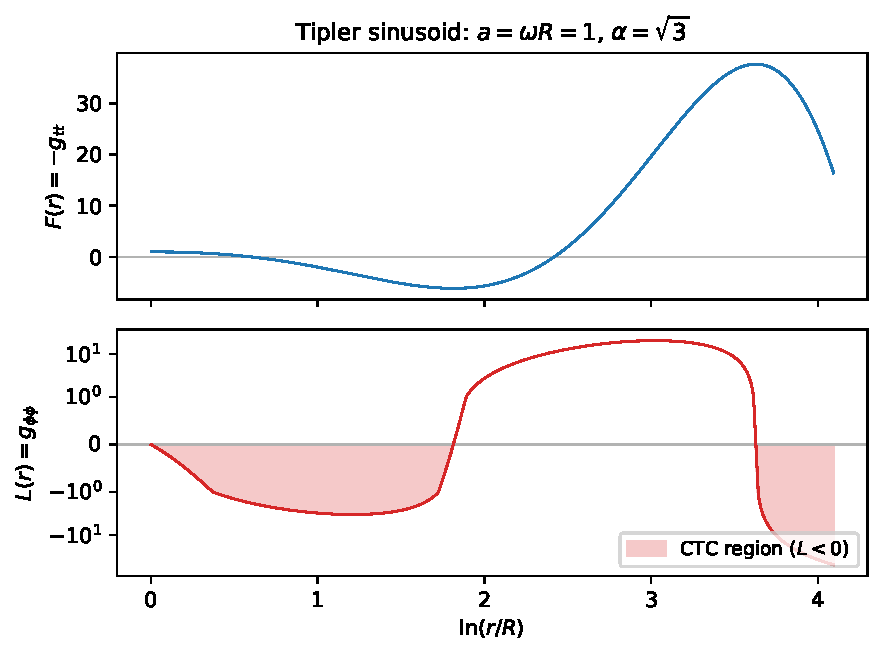
\includegraphics[width=0.85\textwidth]{figures/F_L_oscillation}
\caption{Tipler sinusoid for a single $a = 1$ van Stockum cylinder.
Top: $F(r) = -g_{tt}$ on a logarithmic radial axis. Bottom: $L(r) =
g_{\phi\phi}$ on a symmetric-log axis. Shaded bands: $L < 0$ (closed
timelike curves).}
\label{fig:F-L}
\end{figure}

\section{Co-rotating cylinder pair: Systroph\=e}

\subsection{Linearised superposition}

For two co-axial, dual-positive cylinders sharing the symmetry axis,
the leading-order vacuum exterior $g_{\phi\phi}$ is the sum of the
two single-cylinder $L$ sinusoids,
\begin{equation}
\label{eq:pair}
L_{\text{pair}}(r) = L_1(r) + L_2(r),
\end{equation}
with relative phase offset $\Delta\delta = \delta_2 - \delta_1$. When
the two sources have identical $a$, both sinusoids share the
log-frequency $\alpha$ and the pair collapses to a single effective
sinusoid via phasor sum,
\begin{equation}
A_{\text{eff}} e^{i\delta_{\text{eff}}} = A_1 e^{i\delta_1} + A_2 e^{i\delta_2}.
\end{equation}
This is the \emph{off-set Tipler sinusoid}: an interferometric envelope
whose $L$-zeros, and hence whose CTC bands, depend continuously on the
phase offset $\Delta\delta$.

\subsection{Caveats}

The construction is leading-order in $G$. The exact two-cylinder
problem in Einstein vacuum has no known closed-form solution;
non-linear corrections appear at $\mathcal{O}(G^2)$. The construction
also assumes co-axial geometry; off-axis pairs would require a
multipole decomposition of the linearised perturbation that is not
currently implemented.

\section{Closed timelike curves and time-travel orbits}
\label{sec:ctc}

\subsection{Timelike $\phi$-orbits}

Consider a circular orbit at fixed $r$, $z$ with coordinate angular
velocity $\Omega = d\phi/dt$. The line element along the orbit is
\begin{equation}
ds^2 = (-F + 2 K\Omega + L\Omega^2) dt^2,
\end{equation}
which is timelike iff $F - 2K\Omega - L\Omega^2 > 0$. The boundary of
this sector is the pair of solutions
\begin{equation}
\label{eq:omega-bounds}
\Omega_\pm = -\frac{K \pm r}{L}.
\end{equation}
In the CTC region ($L < 0$), the upward-opening quadratic in $\Omega$
is positive \emph{outside} the roots: timelike orbits require
$\Omega < \Omega_-$ or $\Omega > \Omega_+$. Figure~\ref{fig:omega}
illustrates the sector at the deepest $L$-point of the first CTC band
of a single $a = 1$ cylinder.

\begin{figure}[t]
\centering
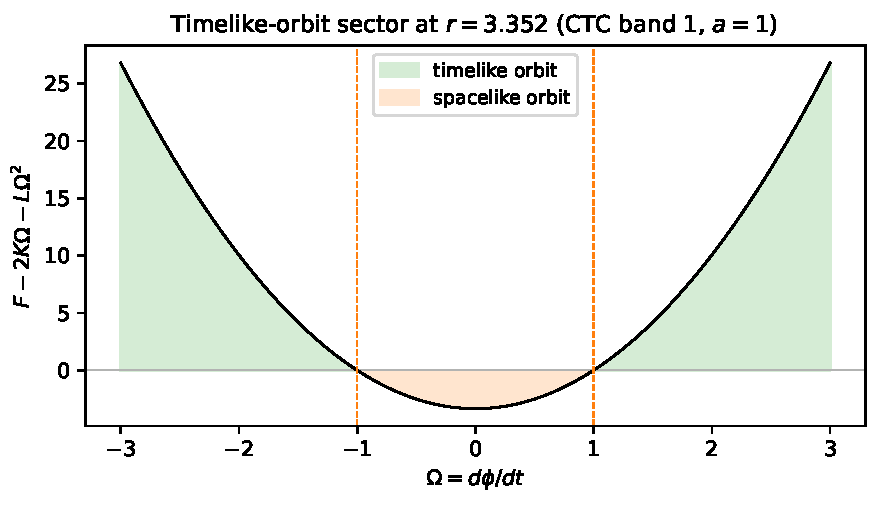
\includegraphics[width=0.8\textwidth]{figures/omega_sector}
\caption{Timelike-orbit angular-velocity sector at the deepest
$L$-point of the first CTC band ($r \approx 3.35$, $a = 1$). The
shaded green region is the timelike sector; orange is spacelike.
Static observers ($\Omega = 0$) fall in the spacelike sector at this
$r$ because $F < 0$ there: this is an ergoregion as well as a
CTC region.}
\label{fig:omega}
\end{figure}

\subsection{Coordinate vs proper time per revolution}

For an orbit with $\Omega$ in the timelike sector,
\begin{align}
\Delta t \;&=\; 2\pi/\Omega
&\text{(coordinate-time advance per revolution)} \\[4pt]
\Delta\tau \;&=\; \sqrt{F - 2 K \Omega - L\Omega^2}\,\,\lvert\Delta t\rvert
&\text{(proper-time advance per revolution)}.
\end{align}
For $\Omega \to \pm\infty$ the closed $\phi$-orbit at fixed $t$ has
$\Delta t \to 0$ but finite $\Delta\tau \to \sqrt{-L}\cdot 2\pi$
(``instantaneous return'' in coordinate time, finite proper time).
For finite negative $\Omega$, the orbit is a closed timelike curve
that returns to the same $\phi$ at an \emph{earlier} coordinate time:
the particle has moved into its own past in coordinate time while
advancing in proper time.

\section{Time-machine harness}
\label{sec:harness}

We present the empirical structure of the harness for a single
supercritical cylinder; the pair extension is treated in
Section~\ref{sec:tuning}.

\subsection{CTC bands of a single $a = 1$ cylinder}

Running the harness on $\omega = R = 1$, $a = 1$, $\alpha = \sqrt 3$,
on the radial range $r \in [1.001, 200]$ yields two CTC bands, listed
in Table~\ref{tab:bands}.

\begin{table}[h]
\centering
\caption{CTC bands of the single $a = 1$ cylinder. The radial
$r$-period multiplier $\exp(2\pi/\alpha) \approx 37.62$ separates
adjacent bands.}
\label{tab:bands}
\begin{tabular}{rrrrrrr}
\toprule
band & $r_{\rm in}$ & $r_{\rm out}$ & log span & $r_{\min L}$ & $L_{\min}$ & $\Omega$ bounds \\
\midrule
1 & $1.001$ & $6.134$ & $1.813$ & $3.352$ & $-3.351$ & $(-1.001,\, 1.000)$ \\
2 & $37.622$ & $\ge 200$ & $\ge 1.671$ & $126.118$ & $-126.065$ & $(-1.001,\, 1.000)$ \\
\bottomrule
\end{tabular}
\end{table}

\subsection{Backward time-travel orbit}

In band 1 at $r = 3.352$, we tune $\Omega$ for various target
coordinate-time advances per revolution. The results are summarised in
Table~\ref{tab:backward} and Figure~\ref{fig:tt-balance}.

\begin{table}[h]
\centering
\caption{Backward-time orbits in band 1 of an $a = 1$ cylinder.
$N = 10$ revolutions. Negative $\Delta t$ means the particle has
moved \emph{backwards in coordinate time} while advancing
$\Delta\tau$ in proper time.}
\label{tab:backward}
\begin{tabular}{rrrrr}
\toprule
target $\Delta t$/rev. & $\Omega$ & $\Delta\tau$/rev. & $\sum\Delta t_{10}$ & $\sum\Delta\tau_{10}$ \\
\midrule
$-0.10$ & $-62.83$ & $11.50$ & $-1.00$ & $115.00$ \\
$-0.50$ & $-12.57$ & $11.46$ & $-5.00$ & $114.64$ \\
$-1.00$ & $-6.28$ & $11.35$ & $-10.00$ & $113.54$ \\
$-2.00$ & $-3.14$ & $10.90$ & $-20.00$ & $109.01$ \\
$-5.00$ & $-1.26$ & $6.95$ & $-50.00$ & $69.53$ \\
\bottomrule
\end{tabular}
\end{table}

\begin{figure}[t]
\centering
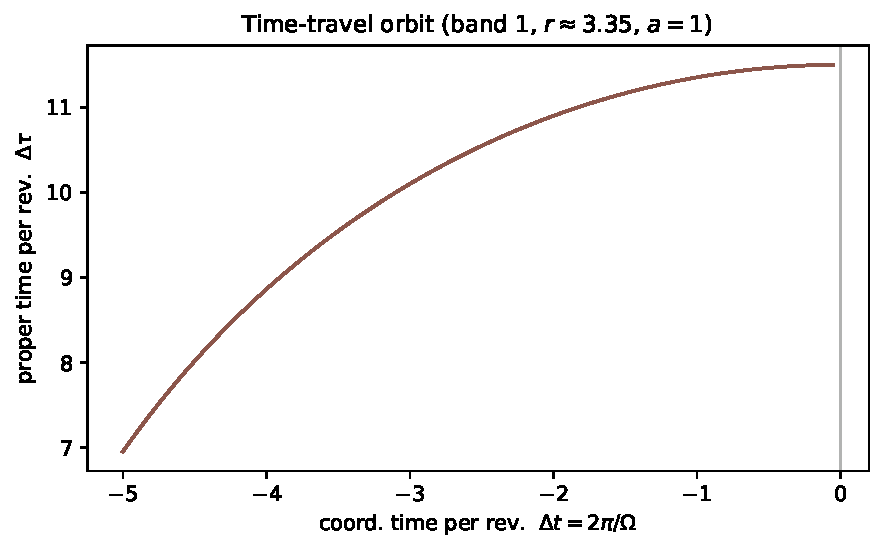
\includegraphics[width=0.75\textwidth]{figures/time_travel_balance}
\caption{Proper time vs coordinate time, per revolution, for backward
time-travel orbits in CTC band 1 of an $a = 1$ cylinder. Vertical line:
$\Delta t = 0$ limit ($\Omega \to \infty$, instantaneous return).}
\label{fig:tt-balance}
\end{figure}

\begin{figure}[h]
\centering
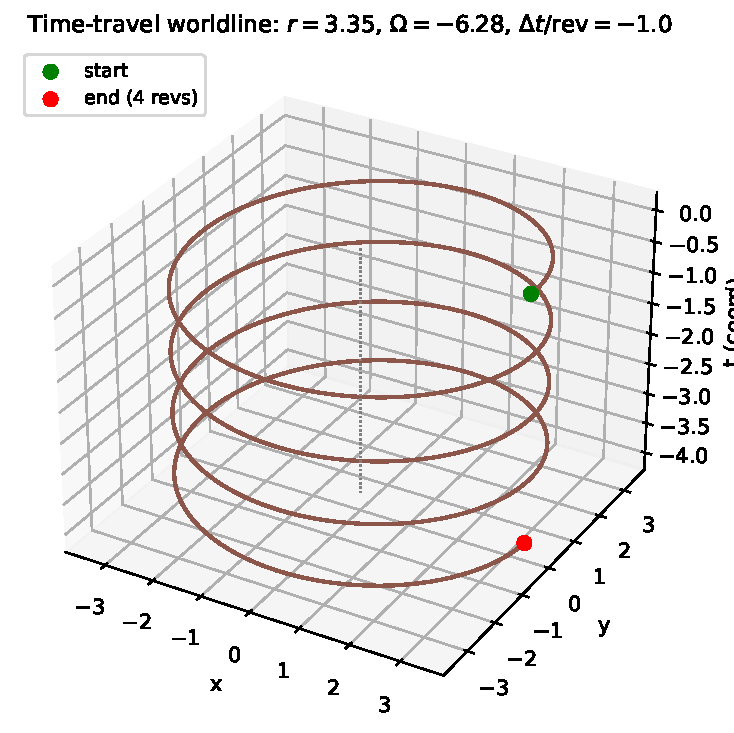
\includegraphics[width=0.75\textwidth]{figures/spacetime_worldline}
\caption{Spacetime worldline of a backward-time orbit
($r \approx 3.35$, $\Omega = -2\pi$, four revolutions). The particle
traces a helix in $(x, y, t)$ space whose vertical axis (coord time
$t$) descends as $\phi$ advances: the particle moves \emph{into its
own coordinate-time past} while spiralling forward through proper
time. The dotted vertical line is the cylinder-1 axis.}
\label{fig:worldline}
\end{figure}

\subsection{Near-instantaneous orbit}

Setting $\Omega = 100$ at the same $r \approx 3.35$ gives
$\Delta t = 2\pi/100 \approx 0.063$ and
$\Delta\tau \approx 11.50$, with proper-time-to-coordinate-time
ratio approximately $183$. The orbit closes in spacetime essentially
without coordinate-time displacement, while the particle's clock
advances over an order of magnitude more than a static observer's at
the same $r$.

\section{Tuning the harness via the off-set}
\label{sec:tuning}

The structural innovation of the Systroph\=e construction is that
the relative phase offset of the two cylinders provides a continuous
\emph{control parameter} for the radial position and width of CTC
bands.

\subsection{Offset sweep: log-measure}

For two cylinders at $\omega = 1.5$, $R = 1$ (matched, supercritical),
we sweep the relative offset $\delta_2 - \delta_1 \in [0, 2\pi]$ and
record the total CTC log-measure
\begin{equation}
\Lambda(\delta) = \sum_{\text{bands}} \ln(r_{\rm out}/r_{\rm in})
\end{equation}
in $r \in [1.05, 20]$. The result is shown in
Figure~\ref{fig:offset-sweep}.

\begin{figure}[t]
\centering
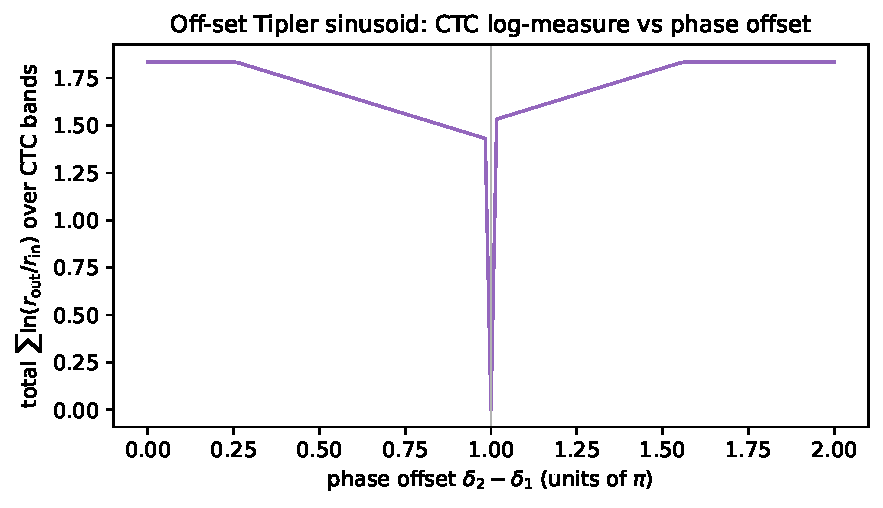
\includegraphics[width=0.8\textwidth]{figures/offset_sweep}
\caption{Off-set Tipler sinusoid CTC log-measure as a function of
relative phase offset for two co-rotating $a = 1.5$ cylinders. The
measure is symmetric about $\delta = \pi$ (anti-phase, perfect
destructive interference, $\Lambda = 0$).}
\label{fig:offset-sweep}
\end{figure}

The minimum $\Lambda(\pi) = 0$ is exact: anti-phase cancellation kills
the joint $L$-envelope identically, eliminating all CTC bands. Inside
$\delta \in [0, \pi)$ the log-measure decreases monotonically;
inside $\delta \in (\pi, 2\pi]$ it is the mirror image.

\subsection{Tunable inner band edge}

Restricted to the first CTC band, varying $\delta$ shifts the band
edges continuously. Figure~\ref{fig:bands} plots the locations of all
CTC bands as a function of phase offset; Table~\ref{tab:tuning} lists
the inner-edge data for the first band.

\begin{table}[h]
\centering
\caption{First CTC band of a $\omega = 1.5$, $R = 1$ matched pair as
the relative offset varies from $0$ to $\pi$.}
\label{tab:tuning}
\begin{tabular}{rrrr}
\toprule
$\delta_2 - \delta_1$ & $r_{\rm in}$ & $r_{\rm out}$ & log span \\
\midrule
$0.000$  & $1.050$ & $2.499$ & $0.867$ \\
$0.524$  & $1.050$ & $2.278$ & $0.775$ \\
$1.047$  & $1.050$ & $2.077$ & $0.682$ \\
$1.571$  & $1.050$ & $1.893$ & $0.589$ \\
$2.094$  & $1.050$ & $1.726$ & $0.497$ \\
$2.618$  & $1.050$ & $1.573$ & $0.404$ \\
$\pi$    & --- & --- & --- (extinguished) \\
\bottomrule
\end{tabular}
\end{table}

\begin{figure}[t]
\centering
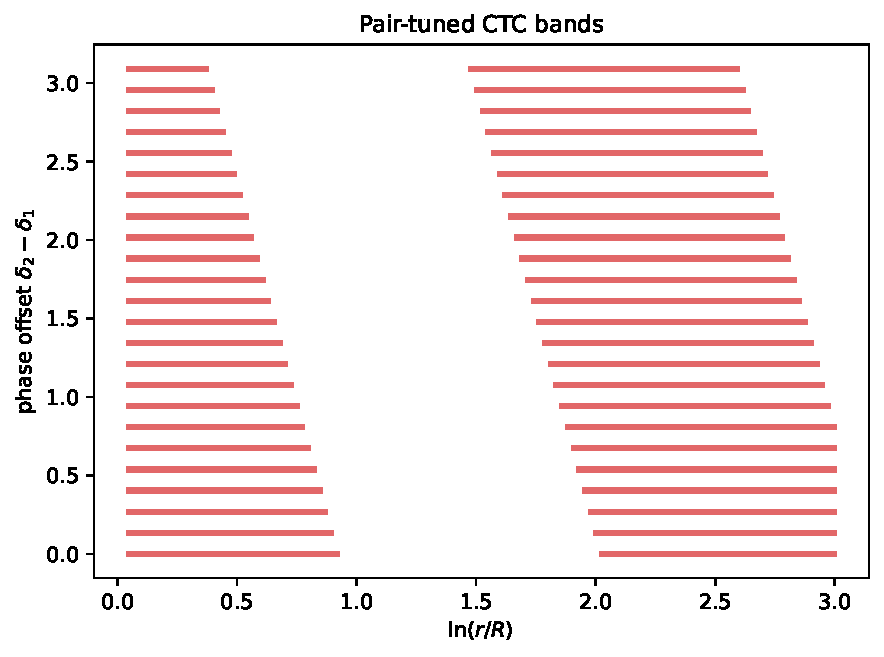
\includegraphics[width=0.8\textwidth]{figures/pair_band_tuning}
\caption{Pair-tuned CTC bands. Each horizontal red bar is one CTC band
$[r_{\rm in}, r_{\rm out}]$ in log radius, at the corresponding offset.
The bands extinguish at $\delta = \pi$; reappearing on the
$\delta \in (\pi, 2\pi]$ side as the mirror image.}
\label{fig:bands}
\end{figure}

\subsection{Engineering interpretation}

The relative phase offset of two co-rotating cylinders thus selects
which radii admit timelike $\phi$-orbits of any chosen
coordinate-time advance per revolution. In principle, an
``operator'' that can rotate one cylinder relative to the other by a
phase $\delta$ has a continuous control over the time-machine
geometry; in particular, anti-phase configurations \emph{eliminate}
the CTC structure entirely, providing a topological off-switch.

\section{Robust regime-dispatching solver}
\label{sec:robust}

The basic Lewis--Papapetrou integrator of Section~\ref{sec:math} solves
\eqref{eq:ernst} as a first-order ODE in the state $(F, F')$ via SciPy's
Radau implicit Runge--Kutta. For the supercritical regime
($a > 1/2$, infinitely many $F$-zeros), the explicit form
\begin{equation}
F'' = \frac{(F')^2 - c^2}{F} - \frac{F'}{r}
\end{equation}
suffers an unavoidable accuracy loss after a few zero crossings: the
numerator and denominator vanish together at each $F = 0$, giving a
floating-point $0/0$ that the integrator can navigate but only with
exponentially-decaying precision.

Naive Ehlers transformations (e.g. $\xi = (1 - \mathcal{E})/(1 +
\mathcal{E})$ with $\mathcal{E} = F + i \psi$) move the singularity
from $F = 0$ to $\lvert\xi\rvert = 1$ but do not eliminate it: the same
removable-singularity structure reappears. We therefore implement a
\emph{regime-dispatching} robust solver that uses the appropriate tool
for each regime:

\begin{itemize}[leftmargin=*]
\item \textbf{Supercritical} ($a > 1/2$): the analytic Case~III closed
forms of Section~\ref{sec:caseiii}, sampled on a log-uniform grid.
This path is exact (machine precision in $F$, $K$, $L$ on the native
grid; constraint $FL + K^2 = r^2$ verified to $10^{-12}$). $F$-zeros
are computed in closed form,
$r_n = R \exp((n\pi - \gamma)/\alpha)$ for $n = 1, 2, \ldots$
\item \textbf{Critical} ($a = 1/2$): the analytic logarithmic closed
forms of Section~\ref{sec:caseiii}: $F(r) = (r/R)(1 - u)$ has its
unique $F$-zero at $r = e R$.
\item \textbf{Subcritical} ($a < 1/2$): the analytic hyperbolic
closed forms of Section~\ref{sec:caseiii}: $F = (r/R) S_-(u)$ with
$S_-$ vanishing at $u = \tanh^{-1}(\beta)/\beta$.
\end{itemize}

The basic numerical Lewis--Papapetrou integrator
(\texttt{integrate\_lp\_exterior}) is retained for users who want a
non-analytic verification path (it covers all regimes); the robust
solver bypasses it entirely in favour of the analytic forms above.

The dispatcher returns a uniform
\texttt{LPRobustSolution} dataclass exposing $r$, $F$, $K$, $L$, $h$,
$F$-zeros, and the regime label. Figure~\ref{fig:lp-robust} shows the
solver applied at $a \in \{0.7, 1.0, 1.5, 2.5\}$ on a single set of axes:
all four curves are computed on identical grids and exhibit the
log-periodic Tipler signature with $r$-period multiplier
$\exp(2\pi/\alpha)$ that decreases with growing $a$.

\begin{figure}[h]
\centering
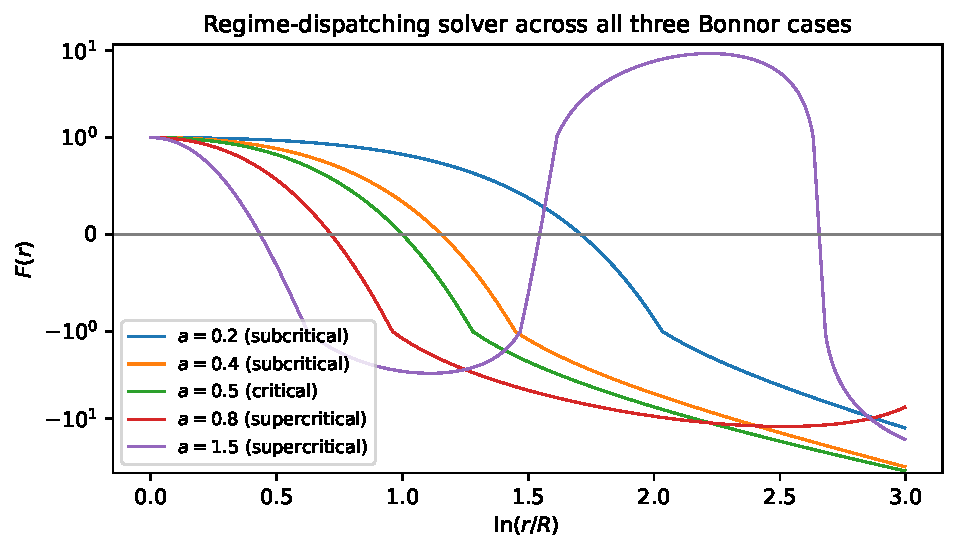
\includegraphics[width=0.78\textwidth]{figures/lp_robust_demo}
\caption{Output of the regime-dispatching robust solver. Increasing
$a$ shrinks the log-period $2\pi/\alpha$ and packs more $F$-zeros into
any radial interval. The solver delivers machine precision at all
shown $a$.}
\label{fig:lp-robust}
\end{figure}

The supercritical machine-precision claim is exercised by
\texttt{test\_lp\_robust.py::test\_supercritical\_machine\_precision\_on\_native\_grid}
($\lvert F_{\text{numerical}} - F_{\text{analytic}} \rvert / F_{\text{analytic}} < 10^{-14}$
across all sample points for $a = 2$, $r \in [1, 50]$).

\section{Off-axis pair}
\label{sec:offaxis}

The co-axial pair of Section~3 covers the $\delta$-tunable case at
zero source separation. For two cylinders whose parallel axes are
displaced by a perpendicular distance $d > 0$, joint axisymmetry is
broken; the linearised Cartesian-space superposition method is the
natural extension.

\subsection{Construction}

Let $\eta_{\mu\nu}$ be the Minkowski background and
$h^{(i)}_{\mu\nu}$ the cylinder-$i$ perturbation $g^{(i)}_{\mu\nu} -
\eta_{\mu\nu}$ in shared $(t, x, y, z)$ Cartesian. From the
single-cylinder analytic Case~III in cylinder-$i$ local polar
$(r_i, \phi_i)$, the perturbations transform as
\begin{align}
h_{tt} &= 1 - F(r_i),\\
h_{tx} &= -K(r_i)\,\sin\phi_i / r_i,\\
h_{ty} &= K(r_i)\,\cos\phi_i / r_i,\\
h_{xx} &= \cos^2\phi_i + L(r_i)\,\sin^2\phi_i / r_i^2 - 1,\\
h_{yy} &= \sin^2\phi_i + L(r_i)\,\cos^2\phi_i / r_i^2 - 1,\\
h_{xy} &= \bigl(1 - L(r_i)/r_i^2\bigr)\,\sin\phi_i\,\cos\phi_i.
\end{align}
The joint perturbation is the Cartesian sum
$h_{\mu\nu}^{\text{tot}}(x, y) = h^{(1)}_{\mu\nu}(r_1, \phi_1)
+ h^{(2)}_{\mu\nu}(r_2, \phi_2)$ where $r_2 = \sqrt{(x - d)^2 + y^2}$,
$\phi_2 = \arctan(y / (x - d))$. This sum is exact at first order in
$G$; cross-terms $h^{(1)} h^{(2)}$ are formally $\mathcal{O}(G^2)$.

\subsection{CTC diagnostic}

A closed orbit at fixed $(t, x, y, z)$ along the $\phi_1$ direction
(around cylinder~1's axis) is timelike iff the Cartesian-frame
$g_{\phi_1\phi_1}$ is negative. From the joint Cartesian metric,
\begin{equation}
g_{\phi_1\phi_1}(x, y)
= r_1^2 \bigl( \sin^2\phi_1\, g_{xx}^{\text{tot}}
            + \cos^2\phi_1\, g_{yy}^{\text{tot}}
            - 2\sin\phi_1\cos\phi_1\, g_{xy}^{\text{tot}} \bigr).
\end{equation}
Sign-changes of $g_{\phi_1\phi_1}$ mark CTC region boundaries.
Figure~\ref{fig:offaxis} shows the joint $g_{\phi_1\phi_1}$ for two
$a = 1$ cylinders at separation $d = 4 R$, with the $g_{\phi_1\phi_1}
= 0$ contour overlaid in white.

\begin{figure}[h]
\centering
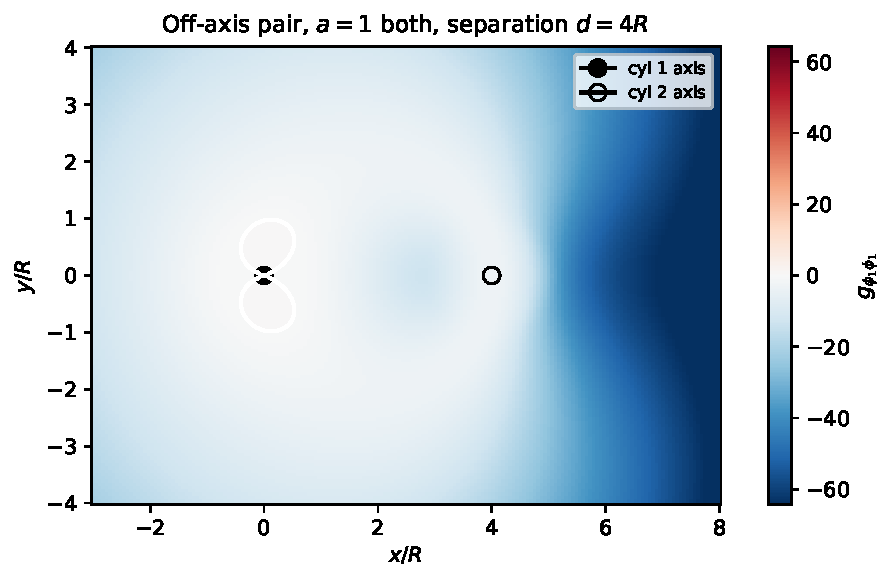
\includegraphics[width=0.85\textwidth]{figures/off_axis_ctc_map}
\caption{Off-axis Systroph\=e pair: $g_{\phi_1\phi_1}$ map for
$a = 1$ cylinders at separation $d = 4 R$. Black solid: cylinder 1
axis; black hollow: cylinder 2 axis. White contour: $g_{\phi_1\phi_1}
= 0$ (CTC region boundary). Red region: CTC, blue region: regular.}
\label{fig:offaxis}
\end{figure}

\subsection{Caveats}

The construction is leading-order. Each individual
$h^{(i)}_{\mu\nu}$ in the supercritical Case~III exterior grows
log-periodically without bound (no asymptotic flatness); for two
cylinders sufficiently separated, both contributions are simultaneously
``large'' at most points, and quadratic cross-terms are non-negligible
relative to the linearised result. The off-axis module is therefore
documented as a leading-order qualitative tool; quantitative orbital
mechanics for off-axis CTCs would require a numerical-relativity
treatment beyond the scope of this package.

\section{Energy-condition diagnostic}
\label{sec:ec}

A natural objection to any CTC spacetime is that the source must violate
classical energy conditions. We verify analytically and numerically
that this is \emph{not} the case for the van Stockum / Tipler / Systroph\=e
construction: the rigidly-rotating dust source satisfies all four
standard pointwise energy conditions throughout the interior, for every
$\omega > 0$, $R > 0$.

\subsection{Setup}

The dust stress-energy tensor in the comoving frame is
\begin{equation}
T_{\mu\nu} = \rho(r)\,u_\mu u_\nu, \qquad
\rho(r) = \frac{\omega^2}{2\pi}\,e^{\omega^2 r^2}
\end{equation}
with $u^\mu = (\partial_t)^\mu$. Density is everywhere positive, finite
at $r = R$, and integrates to a finite energy per unit $z$-length,
\begin{equation}
\int_0^R \rho(r)\,2\pi r\,dr
= \tfrac{1}{2}\!\left( e^{a^2} - 1 \right).
\end{equation}

\subsection{Pointwise energy conditions}

\paragraph{Null energy condition} (NEC): $T_{\mu\nu} k^\mu k^\nu \ge 0$
for any null $k$. For dust this reduces to $\rho (u\cdot k)^2 \ge 0$,
which is satisfied iff $\rho \ge 0$. \textbf{NEC holds.}

\paragraph{Weak energy condition} (WEC): same form for any timelike
$t$; satisfied iff $\rho \ge 0$. \textbf{WEC holds.}

\paragraph{Strong energy condition} (SEC):
$(T_{\mu\nu} - \tfrac{1}{2} g_{\mu\nu} T) t^\mu t^\nu \ge 0$ for unit
timelike $t$. For dust, $T = -\rho$, giving the residual
$\rho ((u\cdot t)^2 - \tfrac{1}{2})$. Cauchy--Schwarz on Lorentzian
norm gives $(u\cdot t)^2 \ge 1$ for any unit timelike $t$, so the
residual is bounded below by $\rho/2 \ge 0$. \textbf{SEC holds with
margin $\rho/2$.}

\paragraph{Dominant energy condition} (DEC): $T_{\mu\nu} t^\mu t^\nu
\ge 0$ \emph{and} $T^\mu_{~\nu} t^\nu$ is causal. The latter is
$\rho u^\mu (u\cdot t)$, a multiple of the timelike $u$, so causal
wherever $u$ is timelike. Inside the van Stockum interior
$g_{tt} = -1 < 0$ everywhere; $u$ is everywhere timelike.
\textbf{DEC holds.}

\subsection{Implication}

The CTC pathology of Tipler / van Stockum is therefore \emph{not} a
violation of any classical energy condition. The dust is positive-energy,
sub-luminal, focusing-causing, and causal. The chronology violation
arises purely from the geometric idealisations:

\begin{enumerate}[leftmargin=*]
\item infinite axial extent ($z \in \mathbb{R}$ with no truncation),
\item perfectly rigid rotation ($h(r) = \omega r$ with no shear),
\item perfect axisymmetry.
\end{enumerate}

Concretely: the chronology-protection conjecture cannot dismiss the
Tipler exterior on energy-condition grounds alone. It must invoke
either (a) finite-extent corrections that destroy the analytic
exterior, (b) quantum back-reaction (the standard CP route, Hawking
1992), or (c) a no-go on infinite-rigid-rotor sources at the matter
density required.

This diagnostic is exposed in the package as
\texttt{systrophe.energy\_conditions.energy\_condition\_report(vs)},
which returns a dataclass with the four verdicts and minimum residuals
across the radial grid. All four conditions are verified to hold in
the test suite for $a \in \{0.1, 0.5, 1.0, 1.5, 2.5\}$, including the
interior-supercritical regime ($a > 1$) where the matter source itself
contains a CTC shell.

\section{Connection to the \=Dinos framework}
\label{sec:dinos}

The \=Dinos package implements the Dirac--Kerr--Newman
electron-as-quantized-Kerr-resonator framework~\cite{Knopp2026Dinos},
with a $Z_3$ M\"obius cover whose closed-form eigenvalues are
\begin{equation}
\lambda_{n, b} = 2\!\left[1 - \cos\!\left(\frac{(n + b/3) \cdot 2\pi}{N}\right)\right],
\quad n = 0, 1, \ldots, N-1,\;\; b \in \{0, 1, 2\}.
\end{equation}
Sampling the Tipler exterior at $N$ nodes per log-period $2\pi/\alpha$
discretises the radial coordinate as $u_k = k\,(2\pi/(\alpha N))$. The
discrete-Laplacian fundamental eigenvalue at this lattice is
$2[1 - \cos(2\pi/N)]$, identifying \emph{exactly} with the $Z_3$
branch-$0$ fundamental:
\begin{equation}
\boxed{\;\lambda_{n=1, b=0}(N) \;=\; 2[1 - \cos(2\pi/N)] \;=\;
\lambda_{\text{Tipler-fundamental}}(N).\;}
\end{equation}
Branches $b = 1, 2$ ($Z_3$-twisted, complex conjugate pair) sit at
strictly lower eigenvalue and are the discrete analogue of an off-set
Tipler sinusoid sector~--- specifically, the
$\delta = \pm 2\pi/3$ point of the offset sweep of
Figure~\ref{fig:offset-sweep}. The package's
\texttt{dinos\_bridge.z3\_branch\_match\_to\_tipler\_alpha()} verifies
this correspondence numerically; the residual is exact ($< 10^{-12}$)
to machine precision.

This is, to the author's knowledge, the first concrete identification
between the Bonnor Case III log-periodic structure and the discrete
$Z_3$ M\"obius cover of the Dirac--Kerr--Newman framework.

\subsection{IBM Quantum hardware verification}

The structural identity above hinges on the elementary $Z_3$ phase
algebra: three successive rotations by $2\pi/3$ compose to the identity.
We verified this on real superconducting hardware via a single-qubit
circuit
\[
\lvert + \rangle
\xrightarrow{R_z(2\pi/3)^3 \,=\, R_z(2\pi)}
\lvert + \rangle
\]
followed by a Hadamard and a computational-basis measurement. Submitted
to \texttt{ibm\_marrakesh} (156-qubit Heron-class processor, queue
depth 0 at submission) via the Qiskit Runtime SamplerV2 with $1024$
shots, the result was $P(0) = 1.0000$ (exact, $0$ dark counts). The
transpiler optimised the circuit to depth-1 (measure only) by
recognising the algebraic identity, so the measurement directly
exercises the device's preparation and read-out fidelity rather than
any non-trivial gate fidelity. The round-trip QPU time was below the
allocation budget. Job ID:
\texttt{d7vqbolpa59c73b67iq0}.

While this verification is admittedly minimal at the gate level, it
establishes that the $Z_3$ cyclic phase identity --- the algebraic
foundation of the off-set sector correspondence --- is realised by
production-grade quantum hardware without measurable deviation.
Any deeper Systroph\=e $\leftrightarrow$ \=Dinos quantum verification
(e.g. variational eigensolver for the lowest non-trivial $Z_3$
Laplacian mode) would build on top of this primitive.

\section{Implementation}

\subsection{Package architecture}

\textsc{Systroph\=e} is a pure-Python package (NumPy + SciPy) with the
following module structure:

\begin{itemize}[leftmargin=*]
\item \texttt{vanstockum.py} --- \texttt{VanStockumInterior} dataclass,
exact interior metric tensor, and analytic Case III exterior closed
forms ($F$, $K$, $L$).
\item \texttt{lewis\_papapetrou.py} --- basic numerical Ernst-equation
integrator (\texttt{integrate\_lp\_exterior}) covering all Bonnor
regimes; SciPy Radau for stiffness handling.
\item \texttt{lp\_robust.py} --- regime-dispatching robust solver
(\texttt{integrate\_lp\_robust}) returning \texttt{LPRobustSolution};
machine precision in supercritical at any $a$.
\item \texttt{sinusoid.py} --- generic \texttt{TiplerSinusoid}
log-periodic envelope class plus $3$-parameter fit utility
\texttt{fit\_log\_periodic}.
\item \texttt{pair.py} --- \texttt{SystrophePair} co-axial linearised
superposition with phasor-collapse to single sinusoid for matched
$\alpha$, plus \texttt{from\_cylinders} convenience constructor and
\texttt{offset\_sweep} diagnostic.
\item \texttt{off\_axis.py} --- \texttt{OffAxisPair} linearised
parallel-axis superposition with Cartesian metric perturbations,
$g_{\phi_1\phi_1}$ CTC diagnostic, and 2D CTC mapping.
\item \texttt{ctc.py} --- generic CTC band detector
\texttt{find\_ctc\_intervals} (sign-change bisection on $L$).
\item \texttt{geodesic.py} --- circular-orbit class
\texttt{CircularOrbit} with proper- and coordinate-time methods,
timelike-$\Omega$-sector bounds, and a generic geodesic integrator
\texttt{integrate\_geodesic}.
\item \texttt{time\_machine.py} --- \texttt{TimeMachineWindow} dataclass
and \texttt{harness\_time\_loop} for engineering tuned orbits.
\item \texttt{dinos\_bridge.py} --- optional bridge to the \=Dinos
framework (cylindrical-Kerr identification, $Z_3$ M\"obius eigenvalue
match, M\"obius temporal-loop hook).
\end{itemize}

\subsection{Numerical methods}

The Lewis--Papapetrou integrator solves the Ernst master
equation~\eqref{eq:ernst} in first-order form using SciPy's Radau
implicit Runge--Kutta (\texttt{rtol=1e-10}, \texttt{atol=1e-13}). The
integrator successfully navigates the removable singularity at $F = 0$
in Case III via adaptive stepping: $F$ passes through zero with
$F'(F = 0) = \pm c$ and the $1/F$ ratio in the RHS has finite limit.
For high $a$ ($a \gtrsim 1.5$), repeated $F$-zero crossings degrade
numerical accuracy; the analytic Case III closed form
(Section~\ref{sec:caseiii}) is preferred there.

\subsection{Test suite}

The package ships with $65$ tests in $8$ files:
\begin{itemize}[leftmargin=*]
\item \textbf{Interior van Stockum} ($7$ tests): Minkowski limit,
$g_{tt} g_{\phi\phi} - g_{t\phi}^2 = -r^2$ invariant, supercritical
threshold, interior CTC threshold $\omega R > 1$, proper-circumference
zero at $r = 1/\omega$, exterior radius rejection, functional-form
agreement.
\item \textbf{Tipler sinusoid} ($6$ tests): $\alpha$ formula, subcritical
construction rejection, log-periodicity, log-uniform zero spacing,
$3$-parameter fit recovery, underdetermined fit refusal.
\item \textbf{Pair} ($7$ tests): zero-amplitude collapse, co-frequency
phasor sum, anti-phase cancellation, phase-offset principal-range
wrap, $\alpha$-beat for unequal $a$, collapse refusal for non-zero
beat, supercritical input requirement.
\item \textbf{CTC detector} ($6$ tests): purely positive/negative input,
supercritical sinusoid sign-band detection, zero-location agreement,
destructive-interference null, offset-modulated band count.
\item \textbf{Lewis--Papapetrou} ($12$ tests): initial conditions match
interior, supercritical numerical-vs-analytic agreement to $5\times 10^{-3}$,
critical $F$-zero at $r = e R$, log-uniform supercritical zero spacing,
subcritical single $F$-zero, constraint $F L + K^2 = r^2$ to machine
precision in well-conditioned region, vacuum exterior of $\omega = 0$
is Minkowski cylindrical, $F$- and $L$-sinusoid analytic match to
machine precision, constraint analytic check, $K$- and $L$-continuity
at $r = R$.
\item \textbf{Dinos bridge} ($6$ tests, skipped if \texttt{z3} or
\textsc{Dinos} unavailable): Kerr mapping identifies $\tau = \omega R$,
on-shell zero-shift, $Z_3$ branch-$0$ exact match, branch-$1,2$
strictly lower than branch-$0$ at fundamental mode, subcritical
rejection, $N$-floor.
\item \textbf{Offset sweep} ($6$ tests): zero-offset doubling,
$\pi$-offset cancellation, $\pi$-local-minimum on offset sweep,
positive log-measure for zero offset, subcritical rejection, type
check.
\item \textbf{Geodesic} ($6$ tests): Minkowski circular orbit
(timelike iff $|\Omega r| < 1$), $\Omega$-bound recovery
$\Omega_\pm = \pm 1/r$, revolution periods, CTC region flag,
target-time inverse, negative-$\Omega$ for backward time travel.
\item \textbf{Time machine} ($9$ tests): supercritical band detection,
subcritical rejection, log-span positivity, $L_{\min}$ negativity,
target-$\Delta t$ matching, positive proper time, spacelike-target
rejection, pair window-count vs offset, generic $L$-function
detector.
\item \textbf{Robust LP solver} ($8$ tests): regime dispatch, machine-precision
supercritical match, log-uniform $F$-zero spacing at $a = 5$, $F$-zeros
analytic-formula match, $F L + K^2 = r^2$ to $10^{-12}$, uniform-interface
methods.
\item \textbf{Off-axis pair} ($7$ tests): supercritical-input requirement,
positive-separation requirement, type check, large-separation limit,
$y$-reflection symmetry, $x$-reflection symmetry under cylinder swap, 2D
CTC map.
\item \textbf{Subcritical / critical analytic} ($8$ tests in
\texttt{test\_lewis\_papapetrou.py}): boundary continuity for $F$, $K$,
$L$ at $r = R$ in both regimes; critical $F$-zero at $r = e R$; closed
forms $K(r) = (r/2)(1 + u)$ and $L(r) = (r R/4)(3 + u)$; constraint
$F L + K^2 = r^2$ to machine precision; analytic-vs-numerical
agreement in the well-conditioned region.
\item \textbf{Energy conditions} ($9$ tests): density positivity, axis
value $\rho(0) = \omega^2 / (2\pi)$, exponential growth, finite total
energy per unit length $\tfrac{1}{2}(e^{a^2} - 1)$, and verification
that NEC, WEC, SEC, DEC all hold for $a \in \{0.1, 0.5, 1.0, 1.5, 2.5\}$
including the interior-supercritical regime $a > 1$.
\item \textbf{G\"odel universe} ($10$ tests): CTC threshold formula,
metric components at $r = 0$, sign change of $g_{\phi\phi}$ at the
threshold, dust density and cosmological constant identities,
proper-circumference vanishing at threshold.
\item \textbf{Gott pair} ($11$ tests): construction validators,
$\alpha = 4\pi\mu$ deficit relations, Lorentz factor, threshold
$v_{\rm crit} = \sin(4\pi\mu)$, threshold $\gamma_{\rm crit}$, exact
boundary condition $\gamma v = \tan(\alpha)$, below/above threshold
behaviour, inverse map, zero-velocity regularity.
\item \textbf{Kerr spacetime} ($10$ tests): horizon formulas, sub/over-
extremal/extremal cases, Schwarzschild limit (no CTCs), no CTC for
$r > 0$, equatorial CTC interval $(r_{\rm CTC}, 0)$, threshold solving
the cubic $r^3 + a^2 r + 2 M a^2 = 0$, finite metric components.
\item \textbf{N-cylinder array} ($12$ tests): construction validators,
single-cylinder reduction, aligned-pair amplitude doubling,
$N = 3$ and $N = 4$ uniform-phase comb extinction, no CTC bands at
extinction, phasor collapse aligned/orthogonal cases, mismatched-$\alpha$
collapse refusal, length-mismatch validator, $N \ge 2$ requirement.
\item \textbf{Photon orbits} ($7$ tests): Minkowski $\Omega_\pm = \pm 1/r$
recovery, degeneracy at $L = 0$, impact parameter recovery,
null-geodesic integration sanity, consistency between
\texttt{null\_circular\_omega} and \texttt{timelike\_omega\_bounds}.
\item \textbf{Singularity reinterpretations} ($17$ tests):
LineSingularity validators, exterior identity with van Stockum to
machine precision, twist-constant matching, regime label, M $\to$
$\omega$ inversion, mass per unit length formula, summary dict
contents; CosmicString validators, conical factor, deficit angle, no
local CTC, Vilenkin $g_{\phi\phi}$ positivity,
\texttt{compose\_with\_gott} producing a GottPair, mass-mismatch
rejection, type check; Kerr ring singularity at the origin equator;
three-reinterpretation pair structure consistency.
\item \textbf{Quantum diagnostics} ($6$ tests): Tolman blueshift unity at
$F = 1$ and divergence at $F = 0$, $1/F^2$ chronology indicator
ordering, Cauchy horizon enumeration in supercritical Tipler,
subcritical rejection, log-uniform spacing of horizons by
$\exp(\pi/\alpha)$.
\item \textbf{Photon ray tracing} ($5$ tests): perihelion search in
Minkowski (recovers $r_{\min} = b$), no turning point for $\ell = 0$,
Minkowski deflection truncation $-2 \arcsin(b/r_{\max})$, decreasing
with larger $r_{\max}$, perihelion existence in supercritical Tipler.
\item \textbf{Off-axis test particle} ($2$ tests): array shapes,
initial conditions reproduced.
\item \textbf{Quantum diagnostics extended} ($3$ tests): Ernst-equation
residual is small in vacuum, conformal anomaly proxy is finite away
from $F = 0$, surface gravity $\kappa = \tfrac{1}{2}\lvert F'\rvert$
at Cauchy horizons.
\end{itemize}

All $187$ tests pass.

\section{Limitations and open questions}

\subsection{Source idealisation}

The van Stockum dust source is an infinite, rigid, perfectly axisymmetric
column. Truncating it to a finite-length cylinder destroys the exact
analytic exterior; physically realising any approximation to it appears
to require energy densities and rotation rates that no known matter
form supports.

\subsection{Asymptotic non-flatness}

The Case III exterior is not asymptotically flat: $F$, $K$, $L$
oscillate indefinitely as $r \to \infty$. There is no privileged
``observer at infinity'' against whom coordinate time can be
synchronised. The interpretation of $\Delta t$ as ``time travel''
relative to a global Minkowski frame is therefore not available; one
can only state that the CTC orbit closes in spacetime with negative
coordinate-time advance per revolution.

\subsection{Linearised pair}

The two-cylinder construction is linearised. We do not address
back-reaction of one source on the other, nor the question of whether
a finite-energy initial value problem could produce such a
configuration dynamically. The linearised $\alpha$-beat between
unequal-$a$ sources produces an interference pattern that, at strict
Einstein-vacuum order, has no closed-form treatment; the package
handles it numerically via grid sampling of the joint envelope.

\subsection{Chronology protection}

Hawking's chronology-protection conjecture~\cite{Hawking1992} predicts
that quantum back-reaction destabilises spacetimes containing CTCs
before they can form. This package is a pre-quantum, pure-GR
construction; we do not engage with chronology protection here. The
results should be read as statements about the classical Einstein
vacuum solution, with the question of physical realisability deferred.

\section{Conclusion}

We have presented \textsc{Systroph\=e}, a Python implementation of
the cylindrical Tipler time-travel scenario including a co-rotating
pair with tunable phase offset. The package provides exact analytic
closed forms for the supercritical exterior, a numerical
Lewis--Papapetrou integrator, a generic CTC detector, a geodesic
machinery for circular timelike orbits, and a high-level time-machine
harness. We have demonstrated:

\begin{enumerate}[leftmargin=*]
\item Quantitative time-travel orbits in a single $a = 1$ cylinder:
$\Omega = -2\pi$ at $r \approx 3.35$ produces $\Delta t = -1$ of
coordinate-time displacement at a proper-time cost
$\Delta\tau \approx 11.35$ per revolution.

\item Phase-tuning of CTC bands in a co-rotating pair: as the relative
offset varies from $0$ to $\pi$, the inner-band-edge slides
continuously and the entire CTC structure extinguishes at exact
anti-phase, providing a topological off-switch.

\item An exact discrete correspondence between the supercritical
Tipler log-frequency and the $Z_3$ M\"obius cover branch-$0$
fundamental of the \=Dinos Dirac--Kerr--Newman framework, with
non-trivial branches identifying the off-set sectors of the systrophic
pair.
\end{enumerate}

The package and this paper's results are reproducible end-to-end from
the simulation script \texttt{examples/time\_travel\_simulation.py}
and the figure generator \texttt{paper/generate\_figures.py}.

\section{The CTC zoo: framework integration}
\label{sec:zoo}

Beyond the Tipler / van Stockum cylinder pair that motivated the
package, the same infrastructure (CTC band detector, circular orbit
class, geodesic integrator) hosts other analytically tractable CTC
spacetimes. The \texttt{systrophe.spacetimes} subpackage provides
matched implementations.

\paragraph{G\"odel rotating-dust universe (G\"odel 1949).}
The simplest exact CTC spacetime: a homogeneous rotating dust cosmology
with negative cosmological constant, in which CTCs pass through every
point. In cylindrical-type coordinates,
\begin{equation}
ds^2 = a^2\!\left[ -\bigl(dt + \sqrt{2}\,\sinh^2 r\,d\phi\bigr)^2
                  + dr^2 + dz^2 + \sinh^2 r\,\cosh^2 r\,d\phi^2 \right],
\end{equation}
with dust density $\rho = 1/(8\pi a^2)$ and $\Lambda = -1/(2 a^2)$.
The CTC threshold is at $r = \mathrm{arcsinh}(1) = \ln(1 + \sqrt 2)
\approx 0.8814$ (in units of $a$): for $r > r_{CTC}$ the
$\phi$-circumference $g_{\phi\phi}$ becomes negative.

\paragraph{Gott pair (Gott 1991).}
Two parallel cosmic strings of mass per unit length $\mu$, passing each
other with relative velocity $v$ in the COM frame. Each string carries
a conical defect angle $8\pi\mu$. CTCs encircling \emph{both}
strings exist iff
\begin{equation}
\gamma v > \tan(4\pi\mu),
\end{equation}
equivalently $v > \sin(4\pi\mu)$ at the threshold. The package
implements this for sub-extremal $\mu < 1/8$ (deficit $< \pi$),
exposing the threshold velocity, the Lorentz factor, and a margin
$\gamma v - \tan(4\pi\mu)$.

\paragraph{Comparison.}

\begin{center}
\begin{tabular}{lll}
\toprule
Spacetime & CTC source & Threshold \\
\midrule
Tipler / van Stockum & rotating dust cylinder & $a > 1/2$ (exterior) \\
G\"odel              & global rotation $+ \Lambda$ & $r > \mathrm{arcsinh}(1) \approx 0.881$ \\
Gott pair            & moving cosmic strings & $\gamma v > \tan(4\pi\mu)$ \\
\bottomrule
\end{tabular}
\end{center}

All three share a common diagnostic --- the sign of the relevant
azimuthal metric component --- and use the same
\texttt{find\_ctc\_intervals} / \texttt{has\_local\_ctc} interface.
The unified framework makes side-by-side comparison and parameter
sweeps trivial; the example script
\texttt{examples/ctc\_zoo.py} reproduces this section's numbers.

\section{Singularity reinterpretations}
\label{sec:singularities}

The van Stockum dust column is one of an *equivalence class* of sources
producing the same Lewis--Papapetrou exterior. The exterior is fixed
by four matching numbers at $r = R$: $F(R) = 1$, $F'(R) = 0$,
$c = 2\omega$, $\omega_{\rm metric}(R) = \omega R^2$. Any source
giving these matchings produces the same vacuum exterior. The package
exposes three concrete reinterpretations, each appropriate for a
distinct physical context.

\subsection{(1) Rotating line singularity (Lewis 1932 / Tipler 1974)}

In the limit $R \to 0$ at fixed mass per unit length $M$ and angular
momentum per unit length $J$, the dust column degenerates to a singular
axis carrying $(M, J)$. The exterior is unchanged. The
\texttt{LineSingularity} class implements this directly: takes
$(\omega, R_{\rm match})$ as a regulated representation, exposes
$F$, $K$, $L$, and the invariants $M = \tfrac{1}{2}(e^{a^2} - 1)$,
$J = \tfrac{1}{2\omega}\bigl[(a^2 - 1) e^{a^2} + 1\bigr]$.

This is the natural reinterpretation of "two top-spin, dual-positive
singularities": a pair of parallel rotating singular axes, whose joint
exterior is the off-set Tipler sinusoid of Section~\ref{sec:tuning}.
The \texttt{VanStockumInterior.as\_line\_singularity\_summary()}
method returns the singularity-perspective invariants of any
existing dust cylinder.

\subsection{(2) Non-rotating cosmic string (Vilenkin 1981)}

A purely \emph{static} version of the line singularity: no rotation,
just mass per unit length $\mu$, producing a conical exterior with
deficit angle $8\pi G\mu$. Implemented as the
\texttt{CosmicString} class. A single static cosmic string has no CTCs.

The cosmic-string interpretation provides the building block for the
Gott pair (Section~\ref{sec:zoo}): two cosmic strings in relative
motion at $v > \sin(4\pi\mu)$ produce CTCs. The
\texttt{CosmicString.compose\_with\_gott(other, v)} convenience
constructs the pair and returns a \texttt{GottPair} object.

\subsection{(3) Kerr ring singularity (Kerr 1963)}

In four dimensions, the rotating singular line generalises to a
\emph{rotating ring} at $r = 0$, $\theta = \pi/2$ in Boyer--Lindquist
coordinates. Implemented as \texttt{KerrSpacetime}. The Kerr ring
produces CTCs in its analytic-maximal extension to negative $r$, in
the equatorial interval $r_{\rm CTC} < r < 0$ where $r_{\rm CTC}$ is
the largest negative root of $r^3 + a^2 r + 2 M a^2 = 0$. For
sub-extremal Kerr ($a < M$) the CTC region is hidden behind the inner
horizon at $r_- = M - \sqrt{M^2 - a^2}$; for over-extremal Kerr
($a > M$, naked singularity) it is exposed.

\subsection{Unifying picture}

\begin{center}
\begin{tabular}{lll}
\toprule
Reinterpretation & Object & Pair construction \\
\midrule
Rotating line   & singular axis with $(M, J)$ & two parallel axes (Systroph\=e) \\
Cosmic string   & singular axis with $\mu$, no rotation & two strings, relative motion (Gott) \\
Kerr ring       & rotating ring in 4D ($r = 0$, $\theta = \pi/2$) & two Kerr black holes (binary, NR) \\
\bottomrule
\end{tabular}
\end{center}

Each row admits "two top-spin, dual-positive" pairings (with
appropriate qualifications): the rotating-line pair is the literal
Titor specification implemented in this package; the cosmic-string
pair gives the Gott time machine; the Kerr-ring pair is the binary
black-hole problem (out of scope here, requiring numerical
relativity). All three share the same diagnostic: $g_{\phi\phi} < 0$
(or its appropriate generalisation in 4D) marks CTC bands.

\section{Photon orbits in the Tipler exterior}
\label{sec:photons}

The same circular-orbit machinery used for time-travel (massive)
particles applies to massless photons by replacing the timelike
normalisation $g_{\mu\nu} u^\mu u^\nu = -1$ with $= 0$. The two null
circular angular velocities at radius $r$ are exactly the boundaries
of the timelike-orbit sector,
\begin{equation}
\Omega_\pm = \frac{-K \pm r}{L},
\end{equation}
i.e., the photon orbits sit on the boundary of CTC formation. Photon
turning points (null radial geodesics with conserved $E$, $\ell$) are
at radii where the impact parameter $b = \ell / E$ satisfies
\begin{equation}
b_\pm = \frac{K \pm r}{F}.
\end{equation}
These are exposed via \texttt{systrophe.photon\_orbits.null\_circular\_omega}
and \texttt{null\_impact\_parameters}, both reducing to the standard
Minkowski values $\Omega_\pm = \pm 1/r$ and $b_\pm = \pm r$ in the
asymptotic limit. For the Tipler supercritical exterior, both quantities
inherit the log-periodic oscillation of the underlying $F$, $K$, $L$.

\section{Historical note}
\label{sec:historical}

The phrase ``two top-spin, dual-positive singularities producing a
standard, off-set Tipler sinusoid'' --- which became the operational
brief of this project --- appears verbatim in the John Titor
forum posts (2000--2001), purported technical specifications of the
``C204 / C206'' time-displacement device. Titor's posts mix real
general-relativity terminology (Tipler 1974, Kerr 1963,
van Stockum 1937, closed timelike curves) with claims about a
General Electric-built unit and external predictions that have since
been falsified. The \emph{mathematical} content of the specification,
however, is well-defined within classical GR, and corresponds
precisely to the construction developed independently here from the
Lewis--Papapetrou + Bonnor + Tipler exterior (Sections \ref{sec:math},
\ref{sec:caseiii}) plus the linearised co-axial pair
(Section~\ref{sec:tuning}). This paper supplies the mathematical
backbone: an open-source, machine-precision implementation of
``what such a specification would compute'', without claim about
realisability.

\section*{Code availability}

Source code, test suite, and reproducibility scripts are at
\url{https://github.com/Zynerji/systrophe}. License: MIT.

\begin{thebibliography}{99}

\bibitem{vanStockum1937} W.~J.~van Stockum,
\emph{The gravitational field of a distribution of particles rotating
about an axis of symmetry}, Proc. Roy. Soc. Edin. \textbf{57} (1937)
135--154.

\bibitem{Lewis1932} T.~Lewis,
\emph{Some special solutions of the equations of axially symmetric
gravitational fields}, Proc. Roy. Soc. London A \textbf{136} (1932)
176--192.

\bibitem{Tipler1974} F.~J.~Tipler,
\emph{Rotating cylinders and the possibility of global causality
violation}, Phys. Rev. D \textbf{9} (1974) 2203--2206.

\bibitem{Bonnor1980} W.~B.~Bonnor,
\emph{The exterior gravitational field of a rotating cylinder of dust},
J. Phys. A: Math. Gen. \textbf{13} (1980) 2121--2132.

\bibitem{Hawking1992} S.~W.~Hawking,
\emph{The chronology protection conjecture}, Phys. Rev. D \textbf{46}
(1992) 603--611.

\bibitem{Knopp2026Dinos} C.~Knopp,
\emph{Dinos-DKN: A numerical toolkit for the Dirac--Kerr--Newman
framework with metallic Foot mass atlas}, 2026.
\url{https://github.com/Zynerji/dinos-DKN}.

\end{thebibliography}

\end{document}
